\chapter{Modélisation}
\label{chap:modelisation}

\section{Choix du formalisme et de la modélisation}
\textit{Écriture des modèles sous forme d'espace d'état}

Notre modélisation sera basée sur les modèles physiques qui décrivent les différents constituants de notre système de procédé : deux moteurs couplés l'un à l'autre par un arbre simple. L'un étant générateur de force mécanique et l'autre générateur de courant afin de faire office de charge (il dissipe son énergie sur une résistance). Il y a aussi un tachymètre couplé à l'arbre principal par un réducteur.
Nos modèles seront donc des modèles de connaissances.

Nous avons choisis de faire une modélisation espace d'état pour différentes raisons. La première est que cette représentation permet de d'étudier facilement la valeur des différents états (l'étude de la stabilité asymptotique, par exemple, est simplifiée en dans un modèle espace d'état). Elle permet aussi de garder les états non observables et non commandables dans le modèle, une modélisation par fonctions de transferts ne le permet pas. Ce choix nous permet aussi, pour la suite, de concevoir un asservissement par retour d'état basé observateur, qui est l'asservissement que nous avons choisi. Le choix d'un modèle de connaissance améliore aussi l'analyse de l'influence des différents paramètres du modèle, ce qui nous permettra d'affiner notre modèle lors des tests sur le système réel. 



\section{Maquette et équations physiques}

Voici, figure \ref{fig:schema0}, un schéma électrique et physique du banc qui fait office de procédé dans notre asservissement.
\begin{figure}[!ht]
\centering
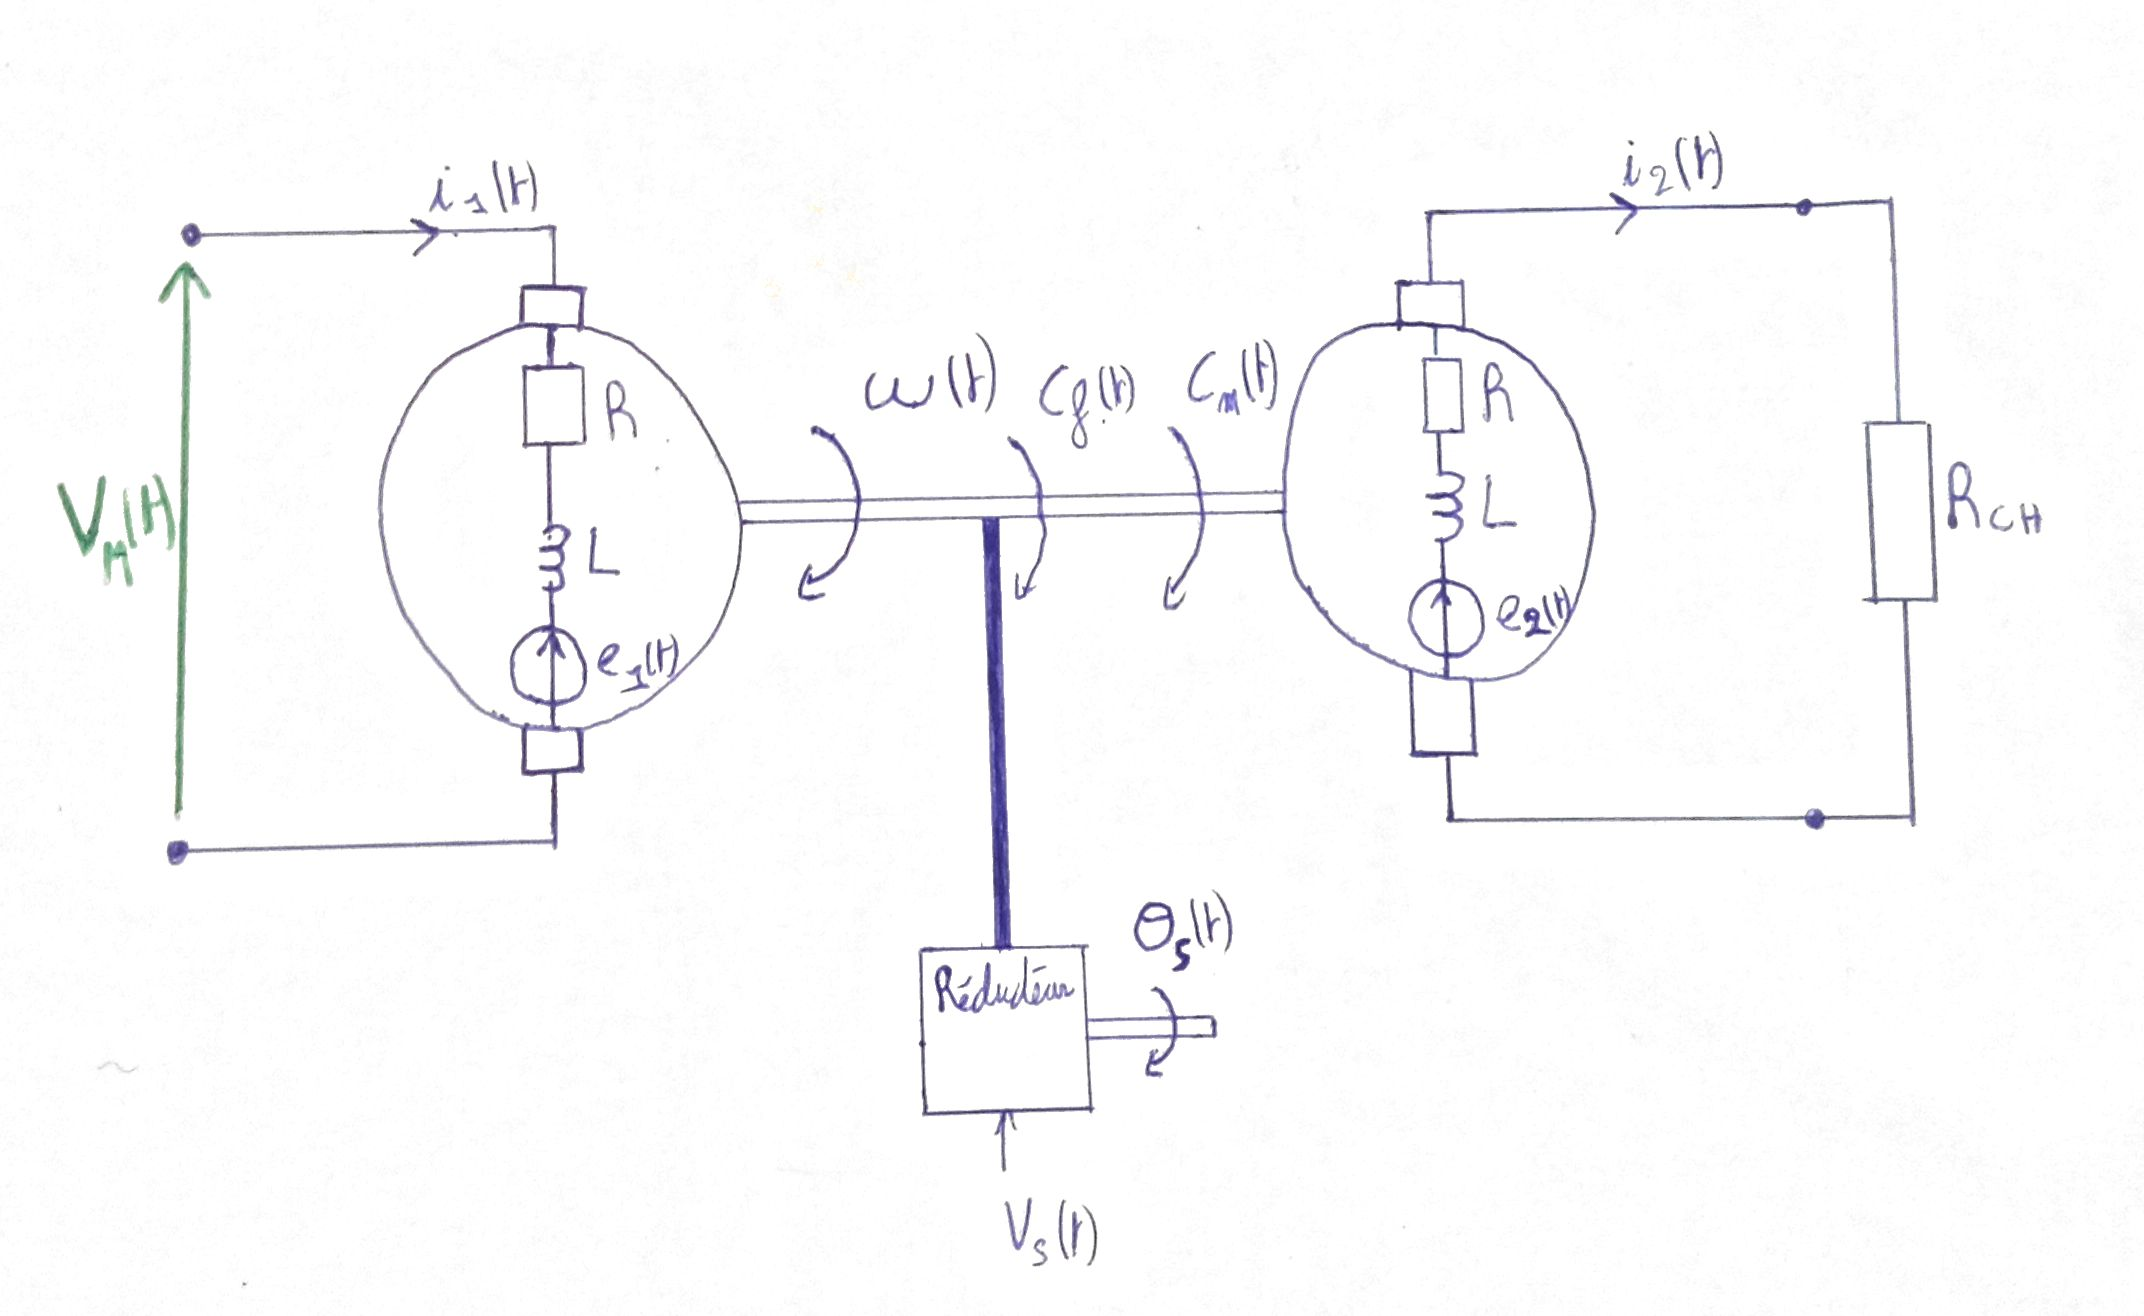
\includegraphics[width=.8\textwidth]{./I/images/schema0.png}
\caption{\label{fig:schema0}Schéma électrique/physique du banc moteur}
\end{figure}
Le circuit électrique de gauche correspond au Moteur à Courant Continue 1 (MCC) qui délivre la puissance mécanique à partir d'une tension d'entrée $V_M$. Celle-ci est l'entrée de notre procédé. Le schéma électrique de droite représente le MCC 2, générateur de puissance électrique qui fait office de charge en alimentant une résistance $R_{CH}$. Entre ces deux schémas électriques, se trouve une représentation de l'arbre, des forces qu'il subit, du réducteur et du tachymètre qui délivre une tension proportionnelle à la position du moteur, c'est le signal $V_s$ que nous étudions en tant que sortie. 


Voici les différentes équations décrivant notre procédé:\\
\noindent\hspace{3mm}\textbullet  \hspace{1mm} Équations des moteurs :
\begin{eqnarray}
V_m(t)  					&=& 	R i_1(t) + L \frac{d   i_1(t)}{d t} + e_1(t) \\
e_2(t) 						&=& 	(R+R_{CH}) i_2(t) + L \frac{d i_2(t)}{d t}
\end{eqnarray}

\noindent\hspace{3mm}\textbullet  \hspace{1mm} Équations banc :
\begin{eqnarray}
J_2 \frac{d \omega(t)}{dt} 	&=&		C_m(t) + C_f(t)		\\
 \frac{d \theta_s(t)}{dt} 	&=&		\omega(t) \\
 e_1(t) &=& K_e \omega(t)\\
 e_2(t) &=& K_e \omega(t)\\
 C_m(t) &=& K_c i_1(t)-K_c i_2(t)\\
 C_f(t) &=& - \mu \omega(t)-C_0(t)\\
 R_{CH}(t) &=& R_{CHn} + rR_{CH}(t) \Delta_1\\
 C_0(t) &=& -sign(C_m(t)C\\
 V_s(t)	&=& K_r K_s \theta_s(t)\\
 V_g(t) &=& K_g \omega(t)
\end{eqnarray}
O\`u :
\begin{description}
\item[$R$] La résistance de l'induit aux moteurs.
\item[$L$] L'inductance de l'induite des moteurs.
\item[$i_1(t),i_2(t)$] Respectivement le courant dans les moteurs 1 et 2.
\item[$e_1(t),e_2(t)$] Respectivement la force électromotrice des moteurs 1 et 2.
\item[$R_{CH}(t)$] Résistance de charge.
\item[ $J_2$ ] Inertie totale (somme des inerties du rotor, du réducteur et de la charge).
\item[$\omega_s(t)$] Position radiale de l'arbre.
\item[$\theta_s$] Vitesse de rotation de l'arbre.
\item[$C_m(t)$] Couple de l'arbre.
\item[$C_f(t)$]  Couple de frottement.
\item[$K_e$] Constante de force électromagnétique.
\item[$K_c$] Constante de couple.
\item[$\mu$] Coefficient de frottement visqueux.
\item[$C_0(t)$] Couple de frottement sec si rotation.
\item[$R_{CHn}$] Résistance de charge nominale.
\item[$rR_{CH}$] Rayon de l'incertitude de la résistance de charge.
\item[$\Delta_1$] Perturbation bornée en $[-1 ; 1]$.
\item[$K_r$] Facteur de réduction.
\item[$K_s$] Constante du potentiomètre.
\item[$K_g$] Constante de la génératrice tachymétrique.
\item[$V_g(t) $] Tension reflétant la vitesse de rotation de l'arbre. Sortie de performance non mesurée. 
\item[$C$] Couple de frottement sec si $\omega(t)$ assez grande.%
%\item[$ $] 
\end{description}



\section{Modèle variant et non linéaire}


\section{Modèle de niveau 0, modèle EE0}
\hspace{5mm} \textbullet \hspace{5mm} Variables d'état :
\begin{equation}
\begin{pmatrix}
\theta_s(t)\\
\omega(t)\\
i_1(t)\\
i_2(t)\\
\end{pmatrix}
=
X(t)
\end{equation}


Pour commencer l'étude avec un espace d'état, nous proposons de poser un premier modèle d'état d'ordre 4. Le vecteur d'état choisit est :
\begin{equation}
X(t)=\begin{bmatrix}
i_1\\
i_2\\
\Omega_m\\
\Theta_m\\
\end{bmatrix}
\end{equation} 
Le modèle d'ordre 4 vaut donc :
\begin{align}
\label{EE0}
\left\lbrace
\begin{aligned}
&\dot{X}(t) = \begin{pmatrix}
-\frac{R}{L}	& 	    0				&   -\frac{K_e}{L}	& 0\\
      0			&  -\frac{(R+R_{ch})}{L}	&	-\frac{K_e}{L}	& 0\\
\frac{K_c}{J_2}	&	\frac{K_c}{J_2}		&	\frac{\mu}{J_2}	&	0\\
0&	0&	1&	0
\end{pmatrix}X(t)+\begin{pmatrix}
\frac{1}{L}\\0\\0\\0
\end{pmatrix}V_m(t)\\
&Y(t) = \begin{pmatrix}
0&	0&	K_g	&	0\\
0&	0&	0	&	K_rK_s\\
\end{pmatrix}X(t)
\end{aligned}
\right.
\end{align}
\section{Espace d'état d'ordre 3, modèle EE1}
\section{Espace d'état d'ordre 2, modèle EE2}
Pour correspondre avec un modèle de comportement, nous allons a nouveau réduire la représentation d'état ~\eqref{EE0} pour obtenir un modèle d'ordre 2. Pour cela, nous allons annuler l'effet des dynamiques des courants $i_1$ et $i_2$ qui sont beaucoup plus grandes que les dynamiques de $\omega$ et $\theta$, qui sont celles que nous sommes capable de mesurer et que nous souhaitons asservir.\\
INVERSER BBBBBBBBBBBBBB !!  
\begin{align}
\label{EE2}
\left\lbrace
\begin{aligned}
&\dot{X}(t) 
=
 \begin{pmatrix}
0 &	1 \\
0	&	-\frac{(K_c K_e)}{J_2 R}-\frac{\mu}{J_2}\\
\end{pmatrix}X(t)
+
\begin{pmatrix}
\frac{K_c}{J_2 R}\\
0
\end{pmatrix} 
V_m(t)\\
&Y(t) = \begin{pmatrix}
0	&	K_g	\\
K_rK_s	&	0	\\
\end{pmatrix}X(t)
\end{aligned}
\right.
\end{align}

